\section{Konzeption}\label{sec:Konzeption}

Das vorliegende Kapitel behandelt die Konzeption des Versuchssystems und des Demosystems, dazu erfolgt zuvor die Festlegung der Anforderungen an das System.

\subsection{Festlegung der Systemanforderungen}\label{sec:anforderungen}

Die grundlegende Anforderung an diese Studienarbeit war es, ein Sprecheridentifikationssystem zu entwickeln, welches über eine Webapplikation bedient werden kann.
Da diese Anforderungsbeschreibung noch viel Spielraum über den Funktionsumfang dieses Systems lässt, werden in diesem Kapitel die Anforderungen an das System genauer spezifiziert.

\begin{itemize}
    \item Das System soll lediglich ein Demosystem darstellen, welches die Machbarkeit eines text-unabhängigen Sprecheridentifikationssystems aufzeigt. Es soll nicht in einem produktiven Umfeld eingesetzt werden können.
    \item Der Datensatz für das System ist zu Beginn festgelegt. Das heißt, es werden nur bereits bekannte Sprecher identifiziert. Zudem können keine neuen Sprecher registriert werden, wodurch das Sprecheridentifikationssystem keine dynamische Erweiterung um Sprecher bereitstellen muss.
    \item Das System beschränkt sich auf das Identifizieren eines Sprechers unter 20 Sprechern.
    \item Zur Authentifizierung eines Sprechers wird ein 20-sekündiger Audio-Clip an das System übermittelt. Der Audio-Clip ist dem System bisher unbekannt, aber in gleichen Bedingungen aufgenommen, wie die bekannten Clips.
    \item Das Sprecheridentifikationssystem sollte Teil des Back-Ends sein. Die Bedienung erfolgt über eine Webapplikation, die mit dem System über eine Schnittstelle kommuniziert.
    \item In der Web-Oberfläche des Demosystems soll der zu authentifizierende Sprecher (einer der 20) und ein Verifikations-Clip ausgewählt werden können. Es soll für jeden Sprecher 5 Clips zur Auswahl geben.
    \item So soll der Nutzer des Demosystems testen können, was passiert, wenn ein zu dem zu authentifizierenden Sprecher passender bzw. unpassender Verifikations-Clip ins System gegeben wird.
    \item Das System soll dem Nutzer dann Informationen über die Identifikations-Verteilung (zu welchem Sprecher passt der Clip zu welchem Prozentsatz) und den Authentifizierungs-Status (\gqq{erfolgreich}/\gqq{nicht erfolgreich}) als Rückmeldung darstellen.
\end{itemize}

\subsection{Konzept Versuchssystem}

\subsubsection{Systemidee}

Aus der Literaturrecherche in Kapitel \ref{stand_der_technik} gehen verschiedene Stimmmerkmale zur Benutzerauthentifizierung hervor.
Die Ergebnisse der dargestellten Untersuchungen unterscheiden sich darin, inwieweit die unterschiedlichen Stimmmerkmale die Stimme repräsentieren bzw. zuverlässig für eine korrekte Authentifizierung sind.

Da die Features \ac{LPC}, \ac{LPCC}, \ac{MFCC} und \ac{dMFCC} die grobe Schnittmenge der Untersuchungen darstellt, werden diese in einer eigens durchgeführten Versuchsreihe getestet und evaluiert.
Hierfür wird ein System entworfen, das die Merkmale aus einem Datenset extrahiert und verschiedene Kombinationen vergleicht.
Das Ziel dieses Systems ist, eine ideale Kombination aus Features herauszufinden.
Ein grober Ablaufplan des Systems ist in Abbildung~\ref{fig:PAP_DemoSystem} dargestellt.
\begin{figure}[H]
    \centering
    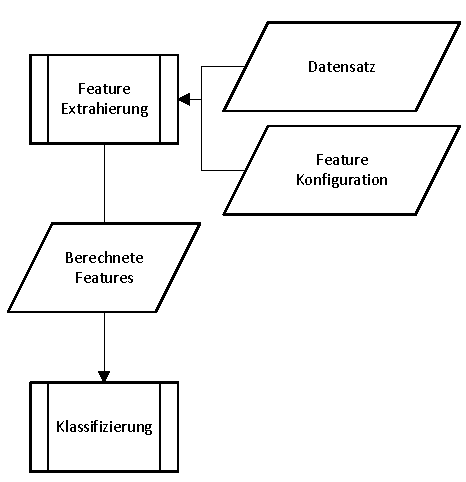
\includegraphics[width=0.6\textwidth, keepaspectratio]{images/PAP_Demosystem.pdf}
    \caption{Ablauf Versuchssystem}
    \label{fig:PAP_DemoSystem}
\end{figure}

% Dazu werden in einem ersten Schritt Konfigurationen definiert, welche die unterschiedlichen Zusammensetzungen der Features beschreibt.
% Anschließend werden alles diese Zusammensetzungen berechnet und durch neuronale Netze klassifiziert.
% Abschließend erfolgt eine Auswertung der verschiedenen Konfigurationen, um eine ideale Konfiguration von Features zu ermitteln

\subsubsection{Feature Kombinationen}\label{sec:FeatureKombination}

Um die Kombinationen zu generieren, werden zunächst die verschiedenen Möglichkeiten definiert und anschließend miteinander kombiniert, was zu über 500 verschiedenen Konfigurationen führt.
Hierzu werden zusätzlich zu den oben genannten Features auch die Anzahl und Länge der Frames definiert.
Für die Anzahl der Frames wurden 10000 und 15000 Frames definiert, für die Länge der Frames 400 und 600 Samples.
Diese Werte berechnen sich aus vorherigen Versuchen, der verwendeten Abtastrate und der gewünschten Trainingsclip-Länge.
Für die Features werden die Anzahl der Features pro Frame auf 13 und 20 festgelegt.
Der Wert 13 ist aus der Literatur abgeleitet \autocite[vgl.][S. 69]{valerio_velardo_mel-frequency_2020}.
Der Wert 20 ist selbstständig ergänzt, um einen Vergleich zu ermöglichen.
Da die Relevanz von \ac{dMFCC} am geringsten ist (s. Abb.~\ref{fig:vergleichFeatureExtraction}), wird hier auf den zweiten Wert verzichtet, um die Anzahl der Konfigurationen zu reduzieren.
Die vorhin genannten Werte sind übersichtlich in der nachfolgenden Tabelle dargestellt.
\begin{table}[H]
    \centering
    \begin{tabular}{l|l}
        \textbf{Bezeichner} & \textbf{Werte}   \\ \hline
        Anzahl der Frames   & 10000, 15000 \\ \hline
        Länge der Frames    & 400, 600     \\ \hline
        LPC                 & 13, 20       \\ \hline
        MFCC                & 13, 20       \\ \hline
        LPCC                & 13, 20       \\ \hline
        delta MFCC          & 13          
    \end{tabular}
    \caption{Übersicht Featurekombinationen}
\end{table}

% \begin{lstlisting}[language=JavaScript,numbers=none,caption=Konfigurationsmöglichkeiten,label=configs]
% Configs = {
%     "amount_of_frames": [10000, 15000],
%     "size_of_frame": [400, 600],
%     "LPC": {
%         "order": [13, 20],
%         "weight": [0, 1]
%     },
%     "MFCC": {
%         "order": [13, 20],
%         "weight": [0, 1]
%     },
%     "LPCC": {
%         "order": [13, 20],
%         "weight": [0, 1]
%     },
%     "delta_MFCC": {
%         "order": [13],
%         "weight": [0, 1]
%     }
% }
% \end{lstlisting}

% Die Werte für die Anzahl und Länge der Frames \codestyle{amount_of_frames} und \codestyle{size_of_frame} berechnen sich aus vorherigen Versuchen, der verwendeten Abtastrate und der gewünschten Trainingsclip-Länge.


% Bei den Features gibt der \codestyle{order} Parameter die Anzahl der Features pro Frame an.
% Der Wert 13 ist aus der Literatur abgeleitet. %TODO CITE
% Der Wert 20 ist selbstständig ergänzt, um einen Vergleich zu ermöglichen.
% Um die Anzahl der Konfigurationen zu reduzieren und da die Relevanz von \ac{dMFCC} am geringsten ist, wird hier auf den zweiten Wert verzichtet.
% Der \codestyle{weight} Parameter gibt lediglich an ob in dieser Konfiguration dieses Feature verwendet werden soll oder nicht.

\subsubsection{Datensatz} \label{sec:KonzeptDatensatz}

Um die unterschiedlichen Kombinationen an Features zu vergleichen wird ein Datensatz benötigt, der mindestens 20 verschiedene Sprecher mit mindestens ca. 15 min unterschiedlichem Audio-Material enthält.
Die Audio-Clips müssen unter gleichen Bedingungen aufgenommen sein und in kompressionslosem WAV-Format vorliegen.

\subsubsection{Feature Extraktion}

In der Feature Extraktion werden die Stimmmerkmale aus den Trainingsdaten extrahiert.
Hierzu müssen die Audiosignale zunächst vorverarbeitet werden (siehe Kapitel \ref{sec:preprocessing}).
In welcher Form die Merkmale extrahiert werden hängt dabei von der aktuellen Konfiguration ab.

\subsubsection{Klassifikation und Evaluierung}\label{sec:KonzeptKlassifikation}

Die Literaturrecherche hat ergeben, dass sich neuronale Netze gut als Klassifikationsmodell eignen (siehe Kapitel \ref{stand_der_technik}). 
Deshalb werden bei der Klassifikation die berechneten Features aus dem Schritt zuvor genutzt, um neuronale Netze zu trainieren, sodass die Feature-Kombinationen bewertet werden können.
Hierbei muss das Netz mehrmals durchlaufen werden, da zu Beginn des Trainings die Struktur zufällig gesetzt wird (siehe Kapitel \ref{sec:neuronaleNetze}).
Anschließend werden die neuronalen Netze mit Testdaten getestet, die nicht in den Trainingsdaten enthalten sind.
Die Auswertung des neuronalen Netzes wird gespeichert und nach Berechnung aller Kombinationen ausgewertet.
Somit soll die beste Kombination gefunden und das damit trainierte neuronale Netz für das Demo-System verwendet werden.

\subsubsection{Software Architektur}
Um eine solide Grundlage für die Entwicklung zu schaffen, wird im Folgenden die Softwarearchitektur für das System entwickelt.
Hierzu wird zunächst basierend auf den vorangegangenen Definitionen ein Klassendiagramm erstellt.
In einem Folgeschritt wird der Ablauf in einem Sequenzdiagramm dargestellt. % optional
\newparagraph
Das Klassendiagramm ist in Abbildung~\ref{fig:klassendiagram-versuchssystem} dargestellt.
Es zeigt die Aufteilung des Systems in mehrere Komponenten (Klassen).
Die wichtigsten Klassen werden nachfolgend kurz beschrieben.
\begin{figure}[H]
    \centering
    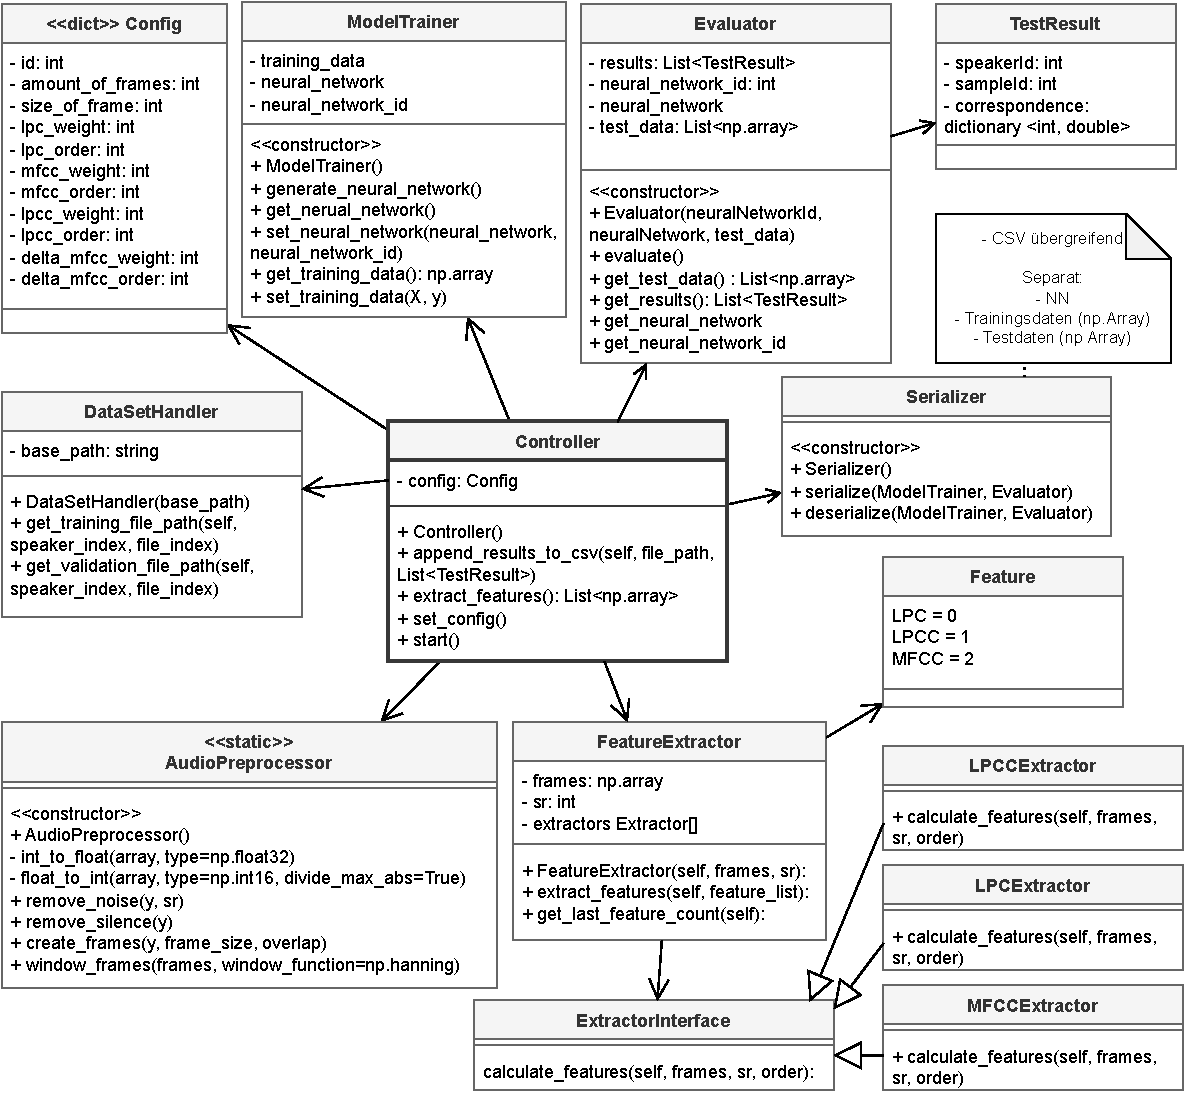
\includegraphics[width=\textwidth, keepaspectratio]{images/klassendiagram-versuchssystem.pdf}
    \caption{Klassendiagramm Versuchssystem}
    \label{fig:klassendiagram-versuchssystem}
\end{figure}\noindent


\noindent \textbf{Controller}\\
Der Controller stellt das zentrale Element dar, von hier werden alle Abläufe gesteuert.
\newline
\noindent \textbf{DatasetHandler}\\
Der DatasetHandler stellt die Verbindung zum Datenset dar und ermöglicht den Umgang mit den Dateien.
\newline
\noindent \textbf{AudioPreprocessor}\\
Der AudioPreprocessor dient im Allgemeinen zur Vorverarbeitung des Audiosignals.
\newline
\noindent \textbf{FeatureExtractor}\\
Mithilfe der FeatureExtractor-Klasse werden variabel die benötigten Audio-Merkmale aus den Audio-Clips generiert. Sie ruft die verschiedenen Implementierungen des ExtractorInterface auf.
\newline
\noindent \textbf{ModelTrainer}\\
Der ModelTrainer generiert und trainiert das neuronale Netz.
\newline
\noindent \textbf{Evaluator}\\
Mit dem Evaluator werden die neuronalen Netze auf ihre Genauigkeit geprüft.
\newline
\noindent \textbf{Serializer}\\
Die Serzializer-Klasse speichert die zu Laufzeit generierten Daten für weitere Untersuchungen.
\newparagraph

In Abb. \ref{fig:sequenzdiagramm-versuchssystem} ist das Sequenzdiagramm dargestellt, dies stellt den Durchlauf einer Konfiguration durch Objekte der verschiedenen Klassen dar.
\begin{figure}[H]
    \centering
    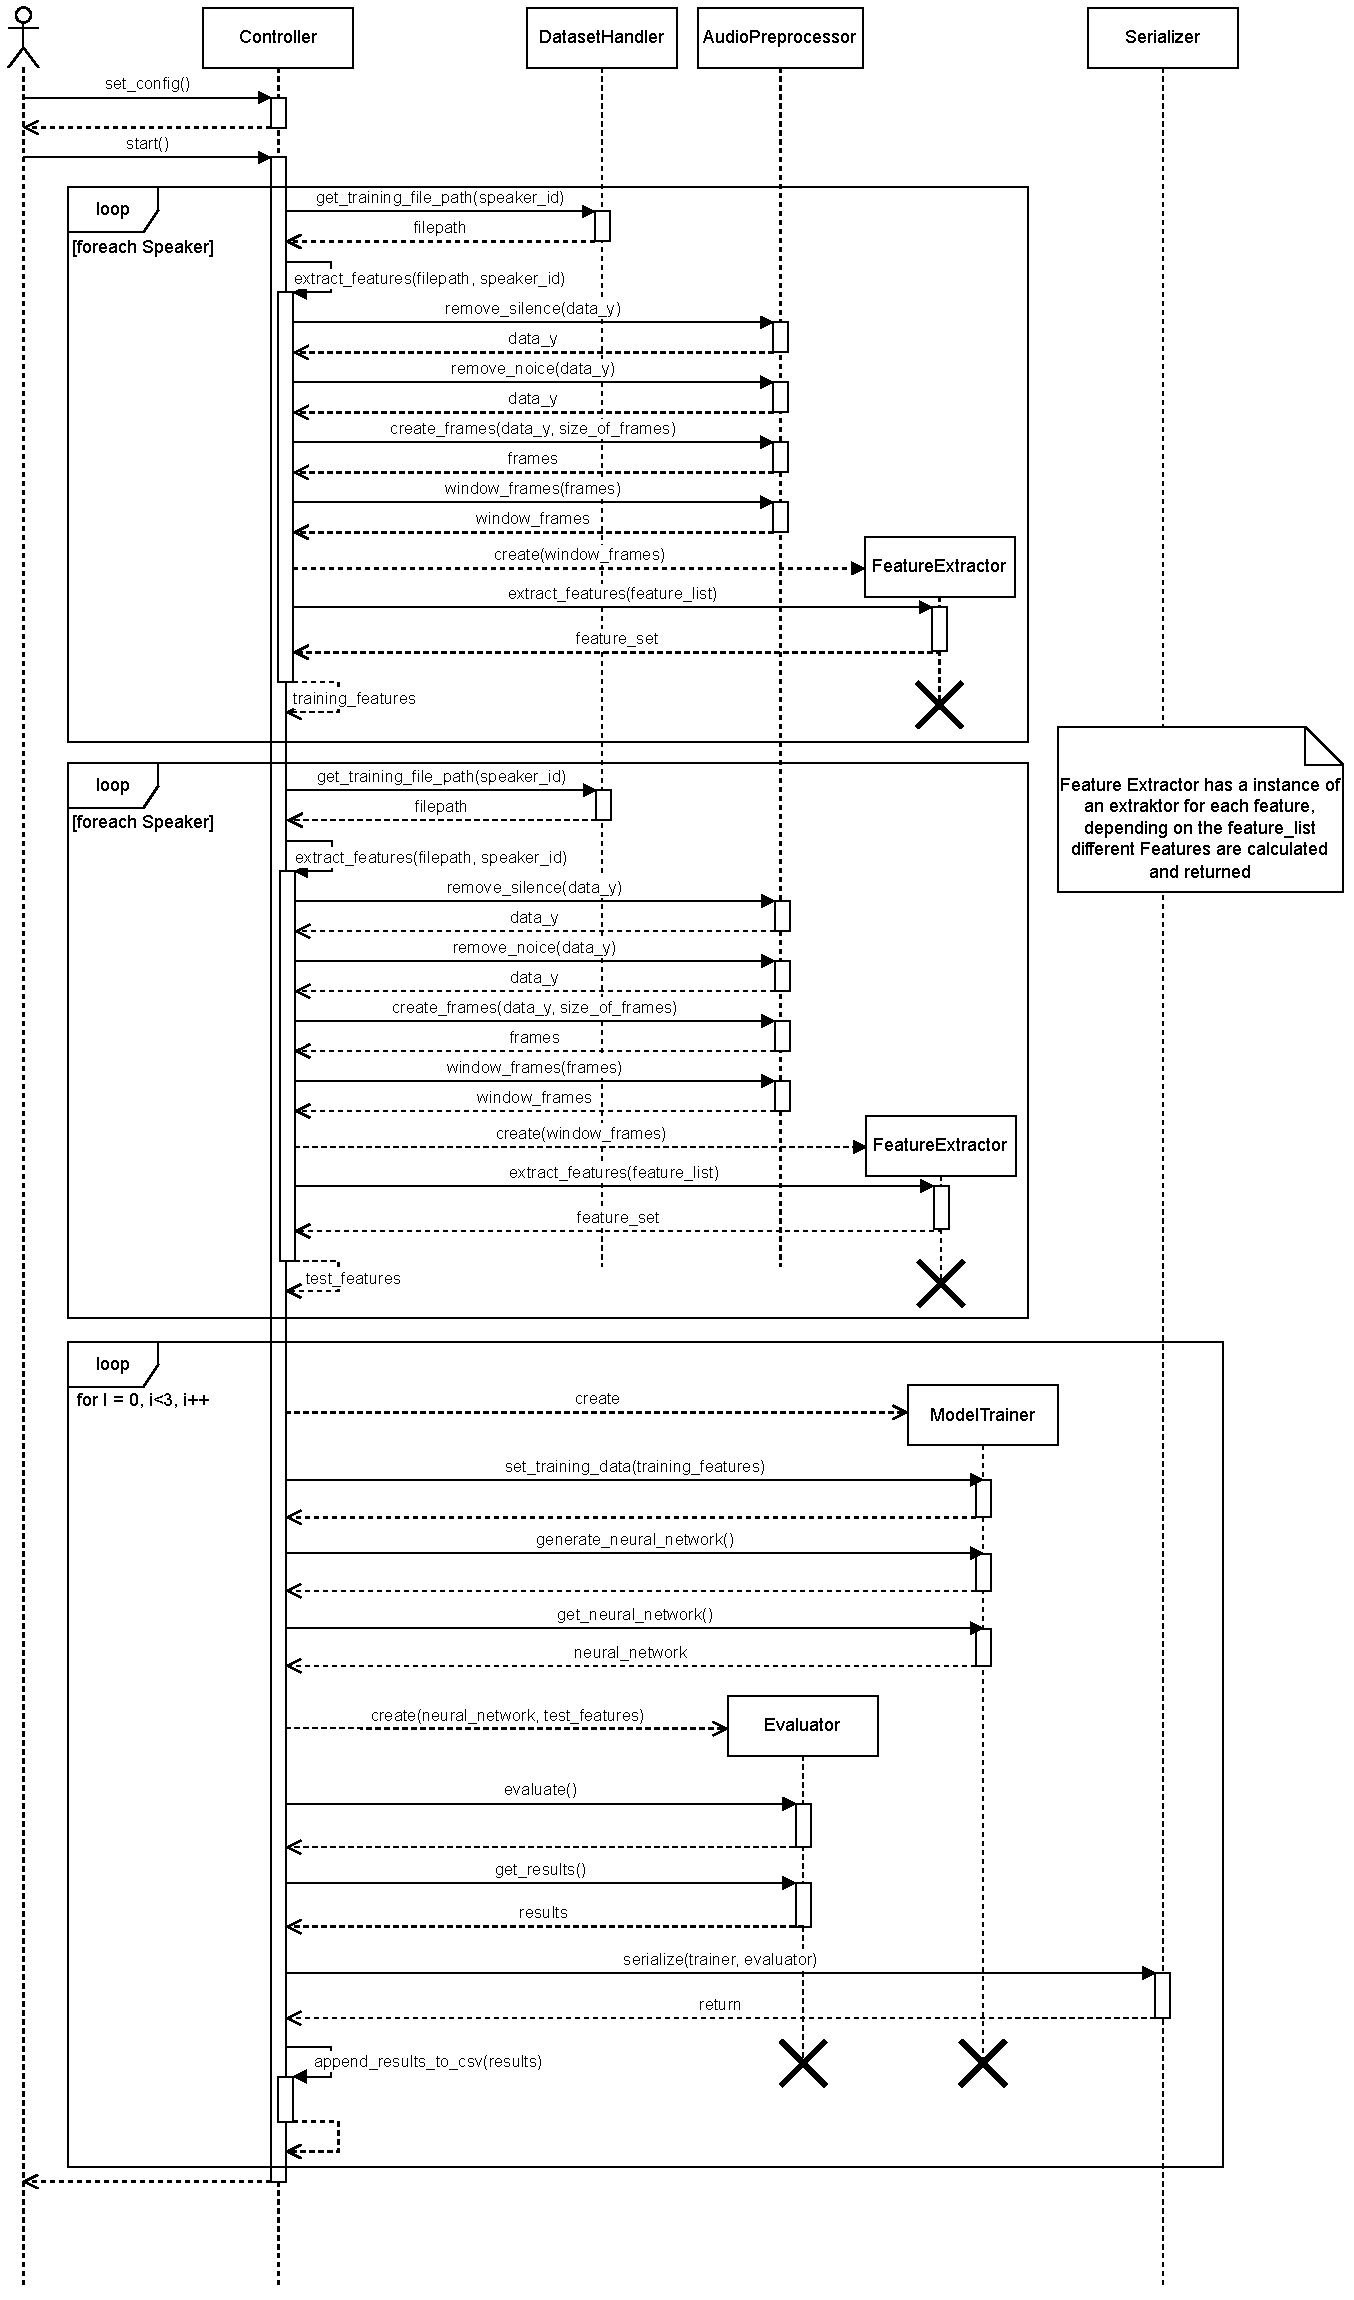
\includegraphics[width=0.82\textwidth, keepaspectratio]{images/versuchssytem_sequenzdiagramm.pdf}
    \caption{Sequenzdiagramm Versuchssystem}
    \label{fig:sequenzdiagramm-versuchssystem}
\end{figure}\noindent




% Beschreibung der Architektur
% GGF Sequenzdiagramm

\subsection{Demosystem}
Ziel des Demosystems ist es, den Authentifizierungsprozess mittels Sprechererkennung zu implementieren und damit die Ergebnisse der Arbeit zu präsentieren.
Aus den Anforderungen in Kapitel~\ref{sec:anforderungen} geht dabei hervor, dass dies als Webapplikation umzusetzen ist.
Dadurch ergibt sich als Basisarchitektur eine Client-Server Architektur, wobei der Client die Weboberfläche und der Server den Authentifizierungsprozess implementiert.
Abbildung~\ref{fig:ArchitectureDemoSystem} zeigt die grundlegende Architektur des Demosystems.

\begin{figure}[H]
    \centering
    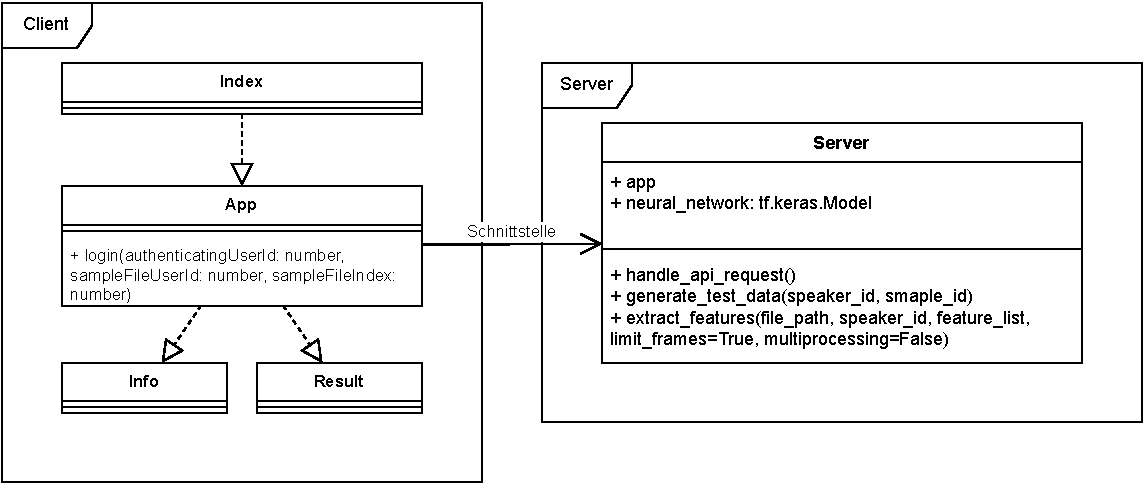
\includegraphics[width=0.9\textwidth, keepaspectratio]{images/Architektur-Demosystem}
    \caption{Architektur Demosystem}
    \label{fig:ArchitectureDemoSystem}
\end{figure}

\subsubsection{Client}
Der Client wird wie bereits erwähnt als Weboberfläche konzipiert.
Dabei stellt er Eingabemöglichkeiten in Form eines Logins bereit, die für das Anstoßen des Authentifizierungsprozesses benötigt werden.
Im Architekturbild geschieht dies über die \textKlasse{App} Komponente.
Über die \textFunktion{login()} Funktion der Komponente wird die Authentifizierungsanfrage an den Server gestellt.

Dabei werden die Daten \textVariable{authenticatingUserId}, \textVariable{sample\-File\-User\-Id} und \textVariable{sample\-File\-Index} über eine Schnittstelle übermittelt.
Da sich das Demosystem auf einen vordefinierten Datensatz beschränkt muss keine Funktion zur Aufnahme neuer Sprechdaten bereitgestellt werden.
Aus diesem Grund werden vordefinierte Audiosequenzen für jeden Sprecher bereitgestellt, die mittels den Variablen \textVariable{sampleFileUserId} und \textVariable{sampleFileIndex} eindeutig identifiziert werden können.

Die Darstellung des Ergebnisses des Authentifizierungsprozesses wird in eine separate Komponente namens \textKlasse{Results} ausgelagert.

Für eine verbesserte Nutzerfreundlichkeit wird zusätzlich eine \textKlasse{Info} Komponente eingebunden, welche die grundlegende Bedienung und Vorgehensweise des Demosystems erklärt.

\subsubsection{Server}
Der Server stellt einen Schnittstellenendpunkt bereit der Authentifizierungsanfragen eines Clients annimmt, verarbeitet und beantwortet.
In Abbildung~\ref{fig:SequenceHandleApiRequest} ist ein exemplarischer Ablauf des gesamten Prozesses modelliert.

\begin{figure}[H]
    \centering
    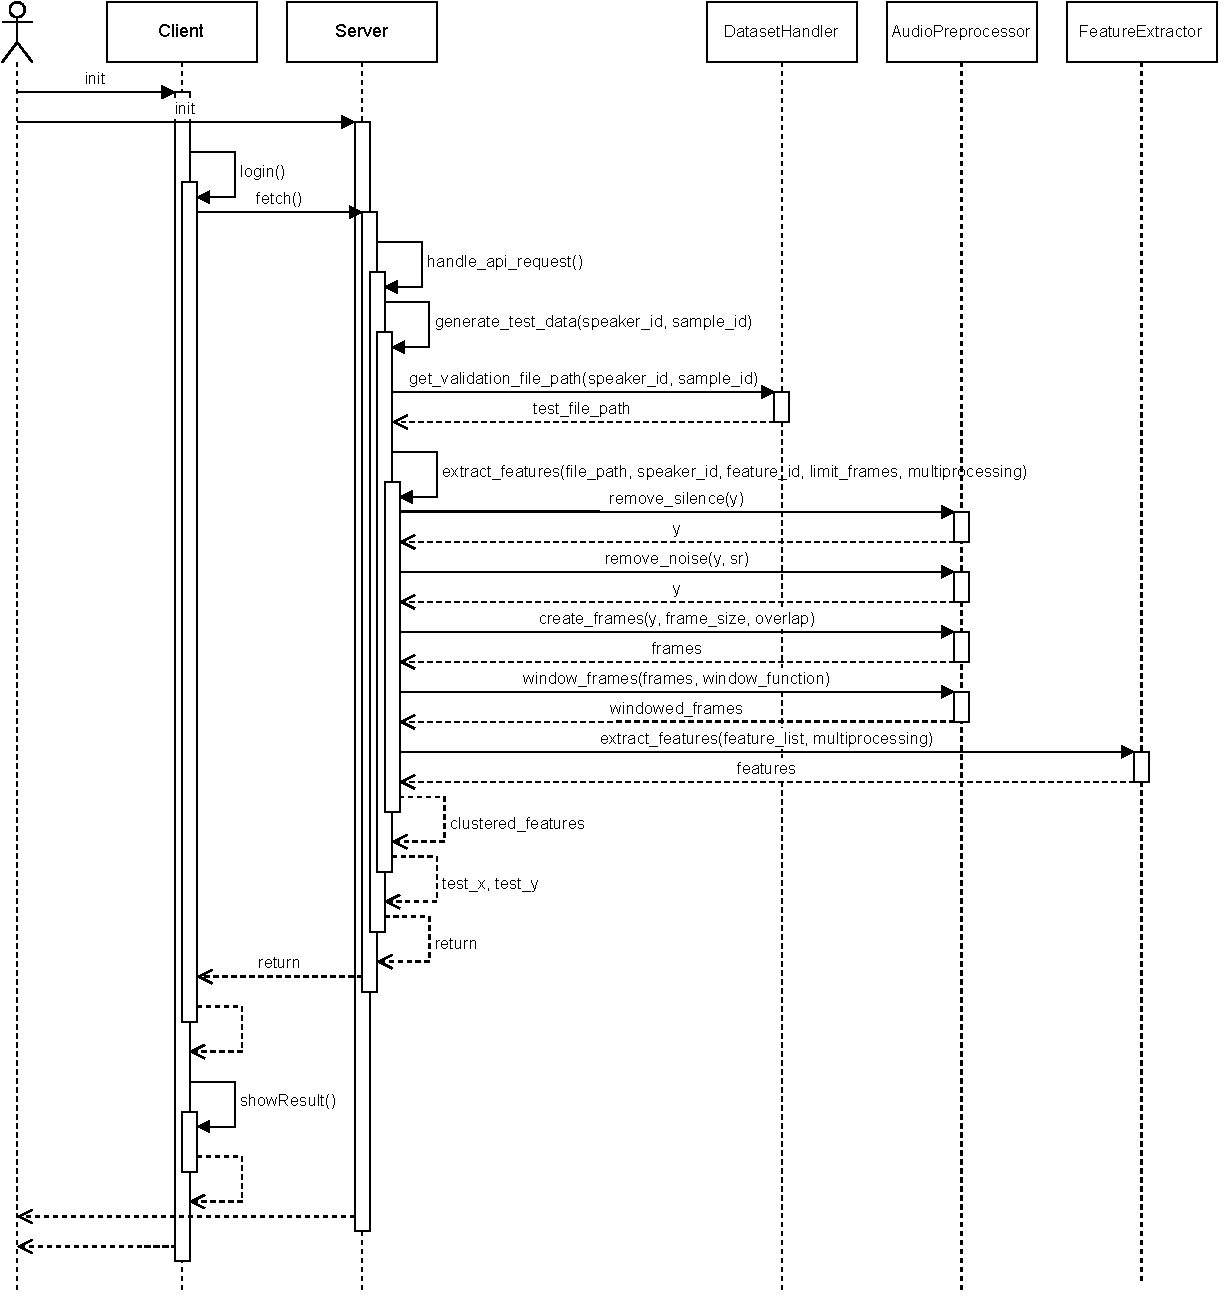
\includegraphics[width=0.9\textwidth, keepaspectratio]{images/SequenzdiagrammClientServer}
    \caption{Sequenzdiagramm login()}
    \label{fig:SequenceHandleApiRequest}
\end{figure}

Eine eingehende Authentifizierungsanfrage wird von der Funktion \textFunktion{handle\_api\_request()} verarbeitet.
Die Klassifizierung der übergebenen Audiodatei verläuft dabei analog zum Versuchssystem, weshalb hier die Komponenten des Versuchssystems (\textKlasse{Dataset\-Handler}, \textKlasse{Audio\-Preprocessor}, \textKlasse{Feature\-Extractor}) innerhalb der Funktionen \textFunktion{generate\_test\_data()} und \textFunktion{extract\_features()} genutzt werden können. % TODO: Evtl. Referenz auf Versuchssystem Konzept

Die Ergebnisse der Authentifizierung werden über die Schnittstelle zurück an den Client gesendet.

\subsubsection{Schnittstellendefinition}
Im Konkreten enthält die Anfrage des Clients die folgenden Informationen:
\begin{itemize}
    \item Zu authentifizierender Sprecher
    \item Index der ausgewählten Sprachdatei
    \item Sprecher der ausgewählten Sprachdatei
\end{itemize}
Die Antwort des Servers beinhaltet die Informationen:
\begin{itemize}
    \item Ermittelte Wahrscheinlichkeit des zu authentifizierenden Sprechers
    \item Authentifizierungsstatus
    \item Ermittelte Wahrscheinlichkeit je Sprecher
\end{itemize}
